\section{Convolution Neural Network}

Convolution is typically used in classical signal and image processing but has recently become popular in neural networks. A classical example is image blurring, where one is given an image $a(x, y)$ which is to be blurred. This blurring is done by averaging neighboring pixels, this average is typically weighted using a 2D Gaussian distribution.

This can be generalized to any input $a(x, y)$ and any weight function $w(x, y)$ by:
\begin{equation}
z(x, y) = (a * w)(x, y) = \int_{-\infty}^\infty \int_{-\infty}^\infty a(i, j) w(x - i, y - j) \partial i \partial j
\end{equation}

Similarly for a discrete image and discrete weight function:
\begin{equation}
z(x, y) = (a * w)(x, y) = \sum_{i = -\infty}^\infty \sum_{j = -\infty}^\infty a(i, j) w(x - i, y - j)
\end{equation}

Both the continues and discrete formulation has some interesting mathematical properties, the convolution operator ($*$) is both commutative and associative. There is also the convolution theorem which combines convolution with the Fourier transformation. While these properties are useful in theoretical work, they have little use in neural networks, it is more the idea behind convolution that is used. In practise neural networks use a finite kernel matrix $w$, and input image $a$. Furthermore, most frameworks use the cross-correlation operator instead of the convolution operator, the difference being that the kernel matrix is flipped. The operation is still called convolution among these frameworks \cite{deep-learning}, this wording is also adopted here and will be used for the rest of the thesis.
\begin{equation}
z(x, y) = (a * w)(x, y) = \sum_{i,\ j} a(x + i, y + j) w(i, j)
\end{equation}

Finally, this thesis uses text as input which only has one dimension, thus a 1D-convolution is used.
\begin{equation}
z(t) = (a * w)(t) = \sum_{i} a(t+r\,i) w(i)
\end{equation}

Convolution has shown to be a very powerful construct, this is primarily because of its locality and its parameter sharing. Locality means that one \textit{pixel} in the output layer only depends on a few \textit{pixels} in the input layer. This makes convolution fast to compute and reasonably easy to parallelize on a GPU. Parameter sharing means that one weight scalar in $w$ is affected by many input and output \textit{pixels}, this causes there to be a lot more data to estimate and optimize the parameter.

\subsection{Padding}
Having a finite input image raises the question of how to deal with the boundaries, where the kernel uses undefined data. In convolutional neural networks, the typical strategy is to either restrict the output image such that all the data is known, this is known as the ``valid'' approach. Alternatively one can add a zero-padding to the input image, such that the valid output image of the extended input image has the same size as the original input image, this is known as the ``same'' approach. Finally, there is the ``full'' approach where the input image is zero-padded as much as what is meaningful. The ``full'' approach is rarely used in neural networks.

\begin{figure}[h]
	\centering
	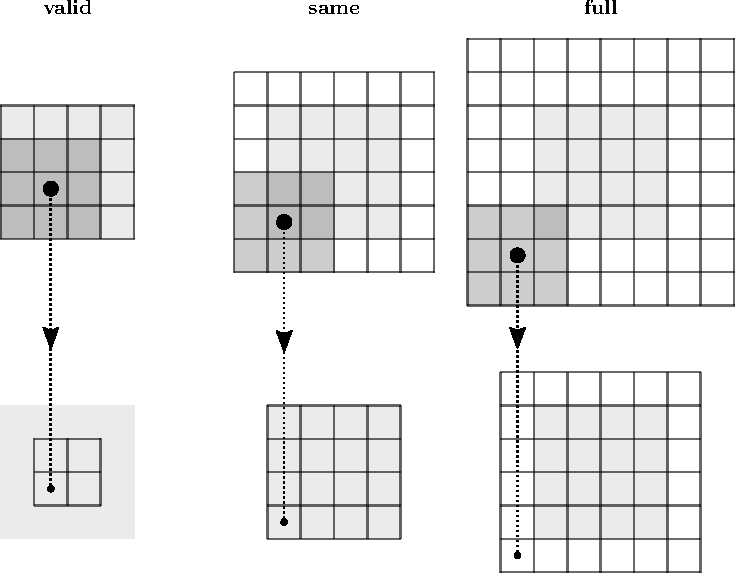
\includegraphics[scale=1]{theory/convolution-padding}
	\caption{Shows 3 padding strategies, known as ``valid'', ``same'', and ``full''.}
	\label{fig:convolution:padding}
\end{figure}

The ``valid'' padding approach is great because it doesn't assume anything about the data, such as if zero is an appropriate padding value. On the other hand, it makes the output image smaller which limits the number of convolutional layers one can apply.

The ``same`` padding approach is great because it doesn't change the output size. However, zero may not be an appropriate padding value. In the ByteNet model presented later ``same`` padding is used because it doesn't change the image size, this is a requirement for residual learning which will be discussed later.

\subsection{Channels}
Ordinary images a separated into 3 colors, red, green, and blue. This concept is generalized to what is called ``channels'', each color is one channel. A convolution will then merge all the channels into a new output image. For the output to have more than one channel, more than one convolution is applied in each layer. This can be expressed as:
\begin{equation}
z_{h_\ell}(t) = (a_{\ell-1} * w_{:, h_\ell})(t) = \sum_{h_{\ell-1}=1}^{H_{\ell-1}} \sum_{i} a_{h_{\ell-1}}(t + i) w_{h_{\ell-1}, h_\ell}(i), \quad \forall h_\ell \in [1, H_\ell]
\end{equation}
where $h_{\ell-1} \in [1, H_{\ell-1}]$ denotes the channel of the input image and $h_\ell \in [1, H_\ell]$ is the channel of the output image.

The use of channels causes a very big increase in the number of parameters, if $w$ has the size $W$ without channels, it now has the size $W \times H_{\ell-1} \times H_\ell$. This increase may seem absurd but in practice channels are extremely powerful. The typical behavior in convolutional neural networks is that each channel will represent some concept. In the first layer, each channel may represent edges in different directions. In the second layer, these edges may be combined to form shapes, such as circular, rectangular, etc.. The last layers may represent ears, noses, and hair, which is finally merged into faces. Neuroscientific research suggests that this is somewhat similar to what is happening in the human brain \cite[chapter 9.10]{deep-learning}.

Similarly for text input one can imagine that letters are transformed into words and words into linguistic meaning. Unfortunately with text, these transformations are much harder to visualize, thus whether or not this is actually what is happening is unknown.

\subsection{Dilated Convolution}

Dilated convolution, also called atrous (with hole) convolution, is an extension on the convolution operator which makes the convolution kernel sparse. The sparseness is described with a dilation rate ($r$), a higher dilation rate means that the kernel is more sparse. A dilated convolution kernel ($w_r$) can be transformed to a dense convolution kernel $w$ by using the Kronecker product (denoted with $\otimes$).
\begin{equation}
w = w_r \otimes \begin{bmatrix}
1      & 0      & \cdots & 0      \\
0      & 0      &        & \vdots \\
\vdots &        & \ddots & \vdots \\
0      & \cdots & \cdots & 0
\end{bmatrix}
\end{equation}

The right-hand side matrix in the Kronecker product is a mostly-zero matrix of size $r \times r$ with just a single $1$ in the top left element. The kernel matrix $w$ is visualized in Figure \ref{fig:convolution:dilation}.

\begin{figure}[h]
	\centering
	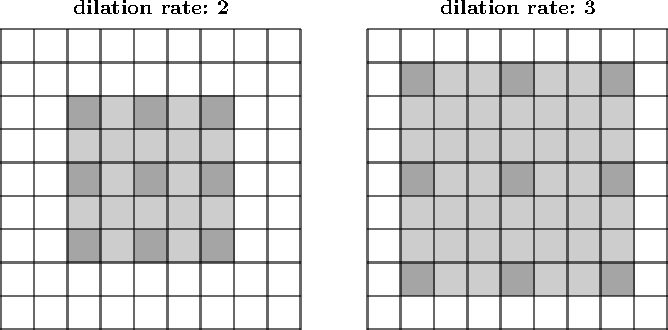
\includegraphics[scale=1]{theory/convolution-dilation}
	\caption{Shows dilated kernel with dilation rate $r = 2$ and $r = 3$.}
	\label{fig:convolution:dilation}
\end{figure}

Obviously converting the sparse kernel to a dense kernel with the Kronecker product is not a very computational efficient implementation. Instead, the convolution (cross-correlation) operator can be modified to support dilation directly.
\begin{equation}
z(x, y) = (a *_r w)(x, y) = \sum_{i,\ j} a(x + r\, i, y + r\, j) w(i, j)
\end{equation}

While dilated convolution doesn't seem particularly useful, it becomes extremely powerful when multiple dilated convolution layers are stacked. For example, if the first layer has no dilation ($r = 1$) and a kernel size of $3 \times 3$, and the second layer has a dilation rate of 3 ($r = 3$) with same kernel size ($3 \times 3$), the visible area of the second layer becomes much larger. This idea is called ``hierarchical dilated convolution'' and is the driving concept in the ByteNet model, it will be discussed later in section \ref{sec:theory:bytenet:hierarchical-dilated-convolution}.

1D dilated convolution with channels can be expressed as:
\begin{equation}
z_{h_\ell}(t) = (a_{\ell-1} *_r w_{:, h_\ell})(t) = \sum_{h_{\ell-1}}^{H_{\ell-1}} \sum_{i} a_{h_{\ell-1}}(t + r\,i) w_{h_{\ell-1}, h_\ell}(i), \quad \forall h_\ell \in [1, H_\ell]
\label{eq:theory:convolution:final-forward}
\end{equation}

The backward pass for \eqref{eq:theory:convolution:final-forward} is derived in Appendix \ref{appendix:backward-pass:dilated-convolution}.
